\chapter{From crowds: Recreating the urban perceptions}
\graphicspath{{Chapter4/plots/} {Chapter5/plots/examples/} {Chapter5/plots/GAN_examples/}}

\label{chap:generation}
\begin{quote}
    ``What I cannot create, I do not understand'' -- Richard Feynman
\end{quote}
Feynman said this insightful quote in context of understanding deeper concepts in physics. If one cannot teach a concept, one does not understand it deeply. 
This notion, albeit disconnected with the premise of my thesis, is as relevant as when it comes to building models of any phenomenon. If a model cannot simulate reality, the model has not really captured the essence of what it is trying to learn. 

In the last chapter, we saw that a large scale crowd poll about perception of urban spaces, can be used to train a machine learning model that can differentiate between an aesthetically pleasing and unpleasant urban image. We also showed that despite the challenges, we can enrich urban data, using certain spatial heuristics. This however did not address an important question, that is, what is the validity of the learnt representation of beauty? Can we use the model's understanding of beauty to our benefit? Is the model actually learning what humans perceive to be the signatures of beauty?
All these questions entail from the final research questions of my dissertation work: 

\noindent\fbox{\begin{minipage}[t][2\height][c]{\dimexpr\textwidth-2\fboxsep-2\fboxrule\relax}
        \textbf{RQ6} \textsl{Can machine learning models based on crowd opinions help us improve real spaces?}
        
        \textbf{RQ7} \textsl{How much do the suggested improvements align with the expectations from the literature or the practitioners?}   
\end{minipage}}
\\

We would try to explore the answers to these questions in this chapter, by systematically dissecting the model of beauty learned in the previous chapter. This, as per the definition framed by Feynman, can be done by first using the model to generate what it ``thinks'' is the notion of urban aesthetic. These generations can be used as recommendations of possible improvements of any given un-aesthetic place. Next we quantify these recommendations using metrics designed around urban design literature. Finally we validated these metrics and recommendations through a user study.  


This approach essentially calls back to the DIKW pyramid approach, where by, to derive insights from data, you first create abstractions that come naturally to the structure of data. In this case, the natural abstraction is the structure of the image itself. You are then supposed to represent the knowledge in the abstractions in the form of metrics that could motivate human wisdom. In this case, we believe that the beauty classifier we saw in Chapter~\ref{chap:quant_perception} has some pertinent knowledge learnt by training on the crowd sourced opinions on beauty. In this chapter, we would develop metrics that operate on this knowledge, to arrive at wisdom inducing insights.


\section{Related work}
Deep learning has been a hot topic and a tool to explore modelling of large datasets in the recent days. The applications of this has seen a steady expansion in the fields other than computer vision and pattern recognition. To list a few, deep learning has made steady headway in natural science allied fields like drug discovery~\cite{gawehn2016deep}, urban science~\cite{pang2017deepcity,cordts2016cityscapes,li2017deep}, health informatics~\cite{ravi2016deep}. The most common forms of deep learning models have been the convolutional neural nets, which we have seen in action in the previous chapter. These convolutional neural networks are essentially layered hierarchical structures of neurons, which can be trained to extract higher dimensional relationships between features in data. This approach has allowed researchers to not only train models to perform simple tasks like detecting objects~\cite{krizhevsky2012imagenet} or detecting faces~\cite{ranjan2017hyperface}, but it has also enabled researchers to quantify much more subjective and intangible properties from images, such as emotions~\cite{kim2013deep},sentiments~\cite{SentiBank} or ambiance of a place~\cite{redi2015like}.

Since the introduction of Generative Adversarial Networks (GANs)~\cite{goodfellow2014generative}, deep learning has been used not only to analyse existing images but also to generate new ones altogether. This family of deep networks has evolved into various forms, from super resolution image generators~\cite{ledig2017photo} to fine-grained in-painting technologies~\cite{pathak2016context}. Recent approaches have been used to generate images conditioned on specific visual attributes~\cite{yan2015attribute2image}, and these images range from faces~\cite{taigman2016unsupervised} to people~\cite{ma2018disentangled}. In a similar vein, Nguyen \emph{et al.}~\cite{nguyen2016synthesizing} used generative networks to create a natural-looking image that maximizes the activation of a specific neuron in the discriminator. This method was used to bring out the latent representation of an image, that maximizes its probability of a particular class. In theory, the resulting image is the one that ``best activates'' the neuron under consideration. In practice, it is still a synthetic template that needs further processing to look realistic.   Finally, with the recent advancement in Augmented Reality, the application of GANs to generate urban objects in simulated urban scenes have also been successfully shown~\cite{alhaija2018augmented}. 

These approaches motivated my work to use GANs, to further investigate the question ``What makes an urban scene beautiful?''. To that extent, I design a framework that utilizes GANs in tandem with the beauty classifier, to reconstruct what the classifier presumes to be beautiful. This is done in a way, that provides an incremental change in a target scene to enhance its beauty. Finally, in accordance with the DIWW framework, I develop metrics to better articulate the knowledge learnt by the model. These metrics are novel and are designed around well known metrics in the literature pertaining to urban design and architecture. 
Finally, I show that this pipeline indeed adds value in the day to day tasks of practitioners of urbanism and the output suggestions around aesthetics of spaces, indeed is perceived to be more aesthetic compared to the input images. 

\section{GAN primer}
A new breed of deep learning algorithms have allowed researchers to generate synthetic data samples, based on knowledge and structure learnt form real data samples ($x$). These family of algorithms are called Generative Adversarial Networks or GANs. GANS work by simultaneously training a Generator $G(z;\theta)$ and a Discriminator $D(x)$ model, who try to out wit each other through training on real samples. The Generator tries to learn to generate the most ``real'' looking synthetic samples by learning the distribution of $x$, and the discriminator $D(x)$ tries to learn to maximize the accuracy on guessing which sample comes from a generator and which comes from the real data. At the peak performance, the generator becomes so good, that the discriminator's accuracy cannot go beyond 50\% mark, implying a totally random guess. This means the Generator 


\begin{figure}[ht!]
    \centering
    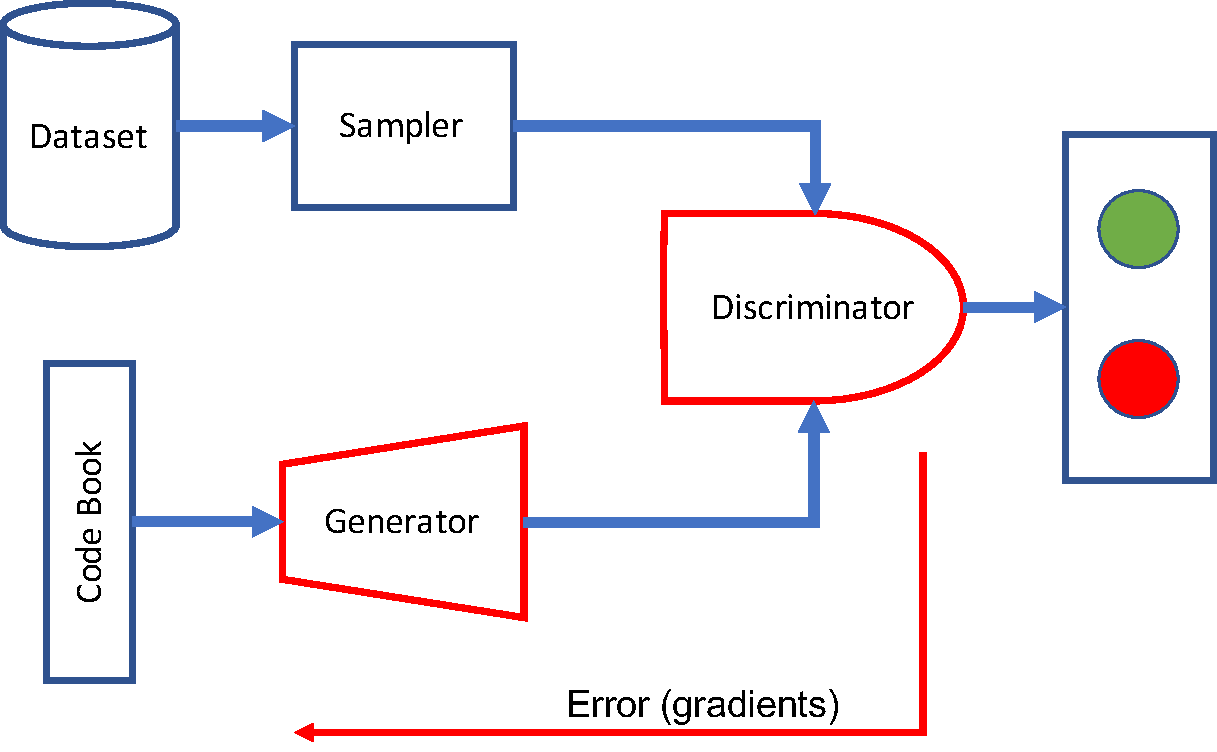
\includegraphics[width=0.7\columnwidth]{GAN_arch.pdf}
    \caption{A simplified illustration of the architecture of a Generative Adversarial Network. The red compunets are trained in tandem, one at a time. The discriminator $D$ tries to maximize accuracy to differentiate between $I$ and the generated version $\hat{I}$. And the Generator $G$ tries to minimize accuracy of $D$ to 50\% thereby making $\hat{I}\approx I$}
    \label{fig:GAN_arch}
\end{figure}

The training of this arrangements of neural networks happen in a lock step mode. 
A simplified version of this arrangement can be found in Figure \ref{fig:GAN_arch}.
The input to the generator $G(z;\theta)$ is initialized using a prior like a gaussian, which essentially creates a codebook of gaussian noise. More formally the discriminator $D(x)$ tries to maximize assigning a correct probability to each sample $x_i$ to be either from the generator $G$ or the real dataset $x$. At the same time, the generator $G$ is trying to minimize the loss$\log(1-D(G(x)))$. Essentially $G$ and $D$ are locked in a two player min-max game with the value function $V(D,G)$ formalized as :

\begin{equation}
\min _{G} \, \max _{D} \, V(D, G)=\mathbb{E}_{\boldsymbol{x} \sim p_{\text { data }}(\boldsymbol{x})}[\log D(\boldsymbol{x})]+\mathbb{E}_{\boldsymbol{z} \sim p_{\boldsymbol{z}}(\boldsymbol{z})}[\log (1-D(G(\boldsymbol{z})))]
\end{equation}

For the premise of my dissertation, I train a generator based on the structure seen at Dosovitsy et.al ~\cite{dosovitskiy2016generating}, on the entire dataset of streetview images obtained in accordance to the strategies discussed in Chapter \ref{chap:quant_perception}. The results of the capacity of this generator to approximate streetview scenes can be see from Table \ref{fig:GanExample}.




\begin{table}\sffamily
    \begin{centering} 
        \begin{tabular}{l*2{C}@{}}
            \toprule
            & Original & Generated \\ 
            \midrule
            & 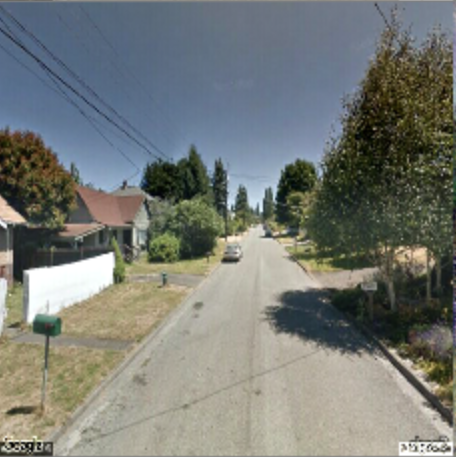
\includegraphics[width=11em]{orig_1} & 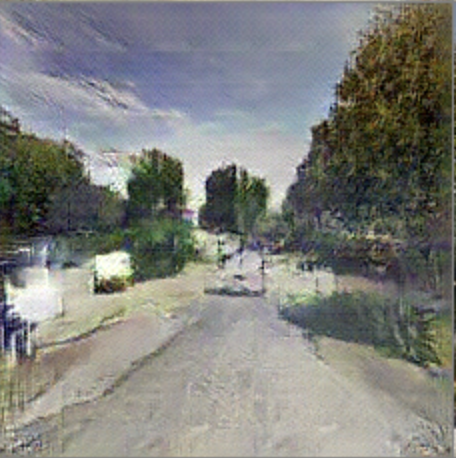
\includegraphics[width=11em]{gan_1} \\ 
            & 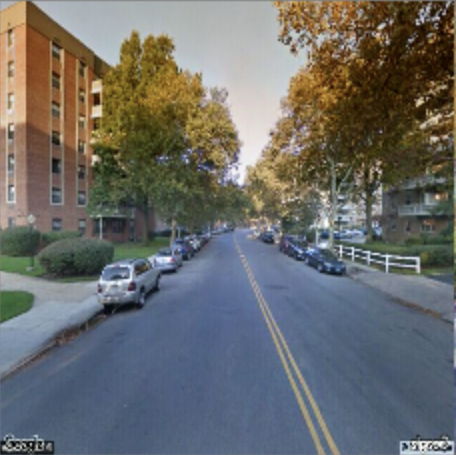
\includegraphics[width=11em]{orig_2} & 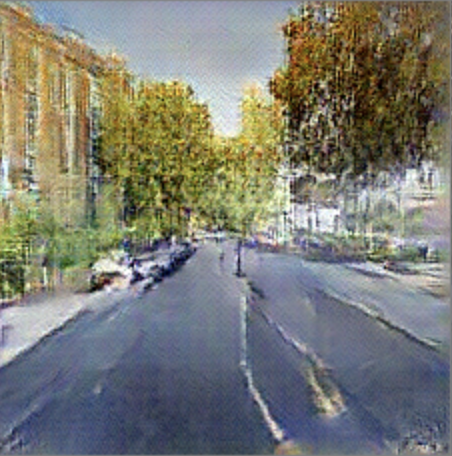
\includegraphics[width=11em]{gan_2} \\ 
            & 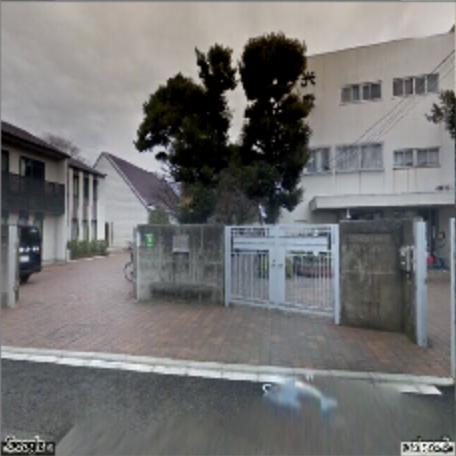
\includegraphics[width=11em]{orig_3} & 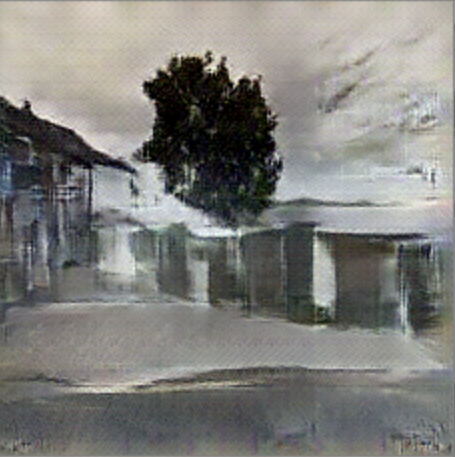
\includegraphics[width=11em]{gan_3} \\ 
            
            \bottomrule 
        \end{tabular}
        \caption{Examples of our generator's outputs. The original scenes and the generated ones are shown side by side.}
        \label{fig:GanExample}
        
    \end{centering}
\end{table} 

\section{Framework Design}



\begin{figure}[t!]
    \centering
    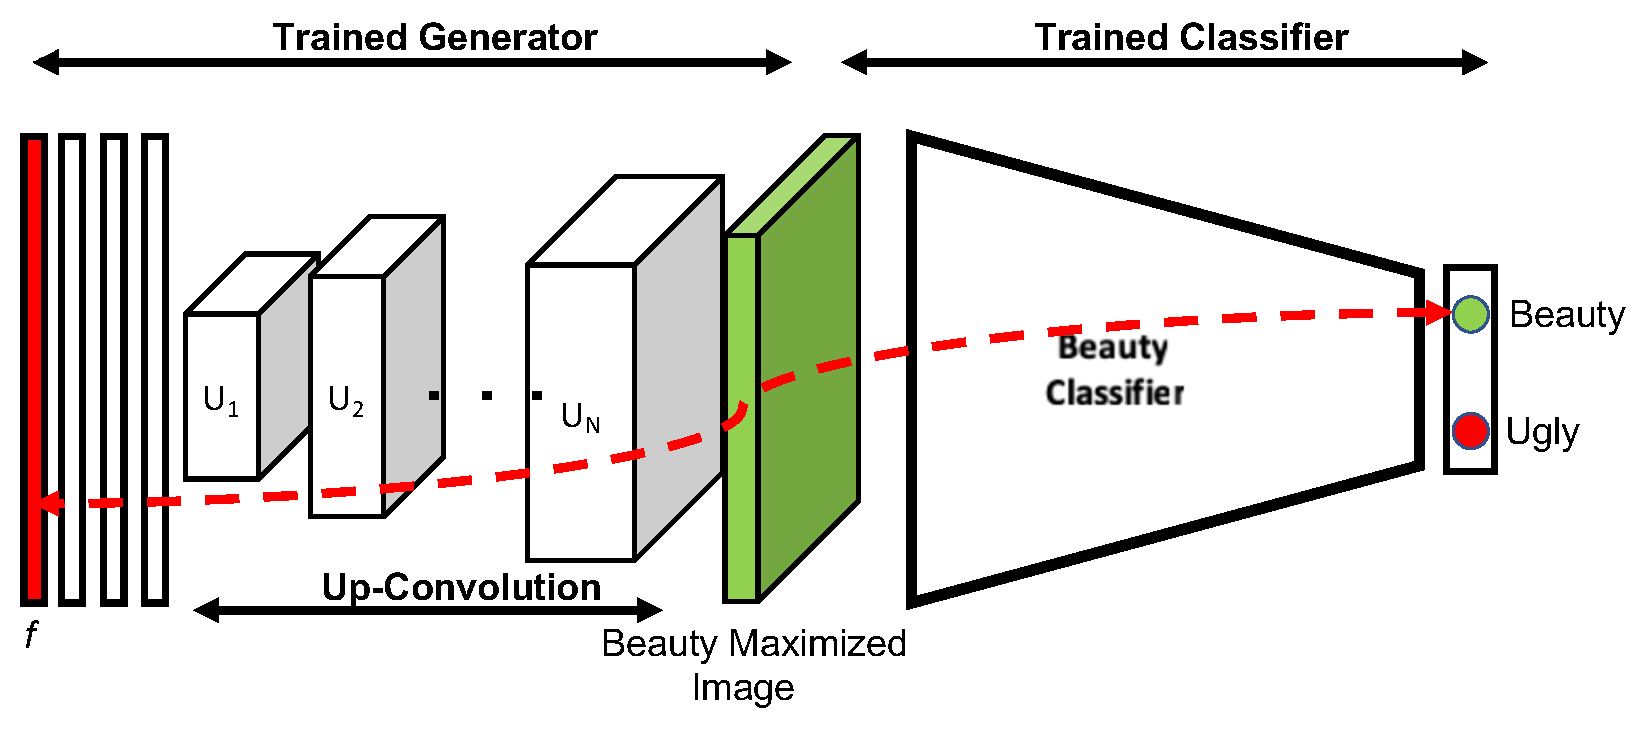
\includegraphics[width=\columnwidth]{AM_arch.pdf}
    \caption{Architecture of the synthetic beauty generator. This consists of a generator of synthetic scenes concatenated with a beauty classifier. The green block is the beauty maximized template $\hat{I_j}$, which is subject to  forward and backward passes (red arrow) when optimizing for beauty.}
    \label{fig:AM_arch}
\end{figure}

\begin{table}[t]
    \resizebox{0.7\linewidth}{!}{
        \begin{tabular}{l|p{8cm}}
            \textbf{Symbol} & \textbf{Meaning}\\
            $I_i$    & Original urban scene \\
            $Y$    & Set of annotation classes for urban scenes (e.g., beautiful, ugly)\\
            $y_i$    & Annotation class in $Y$ (e.g., beautiful) \\
            $\hat{I_j}$ & Template scene (synthetic image) \\
            $I'$ & Target Image \\
            $C$ & Beauty Classifier \\
    \end{tabular}}
    \caption{Notations}\label{notations}
\end{table}

Having the trained classifier at hand and the trained generator of synthetic beautified scenes, the next step is to reconstruct synthetic images using the generator, that maximize the probability of that image being classified as beautiful. The simulated arrangement of this framework can be see in figure \ref{fig:AM_arch} 
As a result, given the two classes: ugly $y_i$ and beautiful $y_j$, the end-to-end model  transforms any original scene $I_i$ of class $y_i$ (e.g., ugly scene) into template scene $\hat{I_j}$ that maximizes class $y_j$ (e.g., beautified template scene). 

More specifically, given an input image $I_i$ known to be of class $y_i$  (e.g., ugly), our technique outputs  $\hat{I_j}$, which is a more beautiful version of it (e.g., $I_i$ is morphed  towards the average representation of a beautiful scene) while preserving $I_i$'s details. The technique does so using the ``Deep Generator Network for Activation Maximization'' (\emph{DGN-AM})~\cite{nguyen2016synthesizing}. Given an input image $I_i$, \emph{DGN-AM} iteratively re-calculates the color of $I_i$'s pixels in  a way  the output image $\hat{I_j}$  both maximizes  the  activation of neuron $y_j$ (e.g., the ``beauty neuron'') and looks ``photo realistic'',  which is done by conditioning the maximization to an ``image prior''. This is equivalent to finding the feature vector $f$ that maximizes the following expression:
\begin{equation}
\hat{I_j} =G( f ) : \underset{f}{\arg\max}(C_{j}(G(f))-\lambda||f||)
\end{equation}
where:
\begin{itemize}
    \item $G(f)$ is the image synthetically generated from the candidate feature vector $f$;
    \item $C_j(G(f))$ is the activation value of neuron $y_j$ in the scene classifier $C$ (the value to be maximized);
    \item $\lambda$ is a $L_2$ regularization term.
\end{itemize}
Here the initialization of $f$ is key. If $f$ were to be initialized with random noise, the resulting $G(f)$ would be the average representation of category $y_j$ (of, e.g., beauty). Instead, since $f$ is initialized with the feature vector corresponding to $I_i$, then the resulting maximized $G(f)$ is $I_i$'s version ``morphed to become more beautiful''.

The input image is also key. It makes little sense to beautify an already beautiful image, not least because such beautification process would result in a saturated template $\hat{I_j}$ in our framework. For this reason, to generate an image that maximizes the beauty neuron in the classifier $C$, we restrict the  corresponding input image to be in class $y_i$ (i.e., ugly scenes as per the divisions in Figure~\ref{fig:Trueskill}). We do the opposite when maximizing the ugly neuron. 

We now have template scene $\hat{I_j}$ (which is a synthetic beautified version of original scene $I_i$) and need to retrieve a realistic looking version of it. We do so by: \emph{i)} representing each of our original scenes in Step 1 (including $\hat{I_j}$) as a 4096 dimensional feature vector derived from the FC7 layer of the PlacesNet~\cite{zhou2014learning}; \emph{ii)} computing the distance (as $L_2$ Norm) between $\hat{I_j}$'s feature vector and each of the original scene's feature vector; and \emph{iii)} selecting the original scene most similar (smaller distance) to $\hat{I_j}$. This results into the selection of the beautified scene $I_j$.


%****************************************
\section{Motifs of urban beauty}
Since original scene $I_i$ and beautified scene $I_j$ are real scenes with the  same structural characteristics (e.g., point of view, layout), we can easily compare them in terms of presence or absence of urban elements extracted by computer vision tools such as SegNet~\cite{badrinarayanan2015segnet} and PlacesNet~\cite{zhou2014learning}. That is, we can determine how the original scene and its beautified version differ in terms of urban design elements. 

\begin{table}\sffamily
    \begin{tabular}{l*3{C}@{}}
        \toprule
        & Original ($I_i$) & Latent Beauty representation ($\hat{I_j}$) & Beautified ($I_j$) \\ 
        \midrule
        & 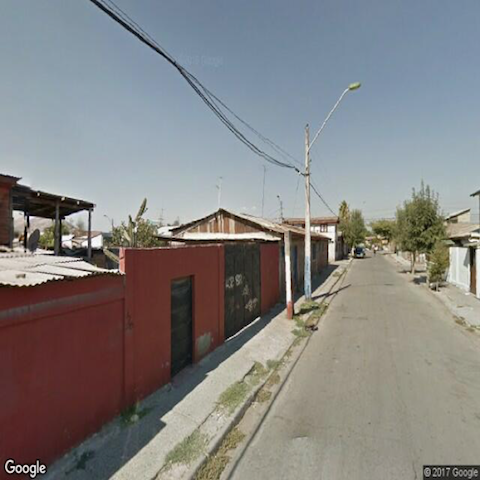
\includegraphics[width=11em]{u_9.png} & 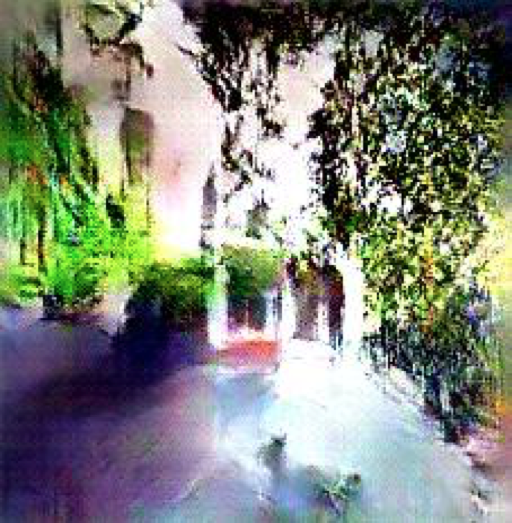
\includegraphics[width=11em]{t_9.png} &  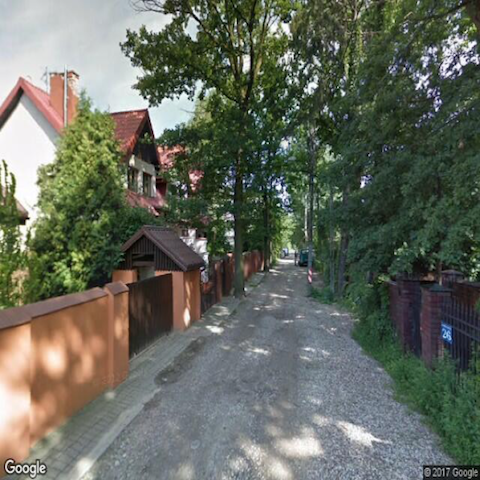
\includegraphics[width=11em]{b_9.png} \\ 
        %		& 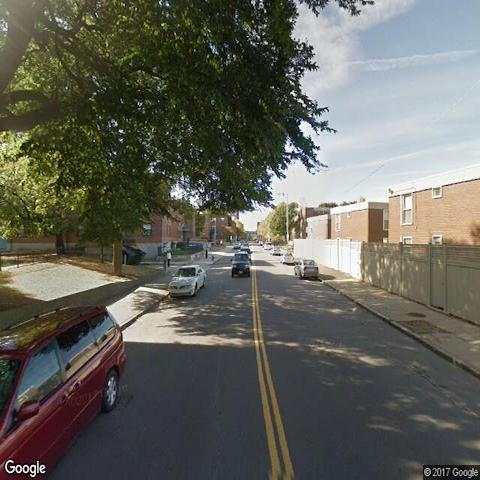
\includegraphics[width=11em]{Plot/examples/u_1} & 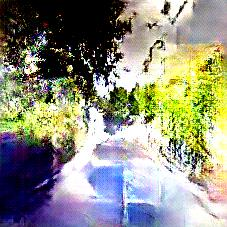
\includegraphics[width=11em]{Plot/examples/t_1} &  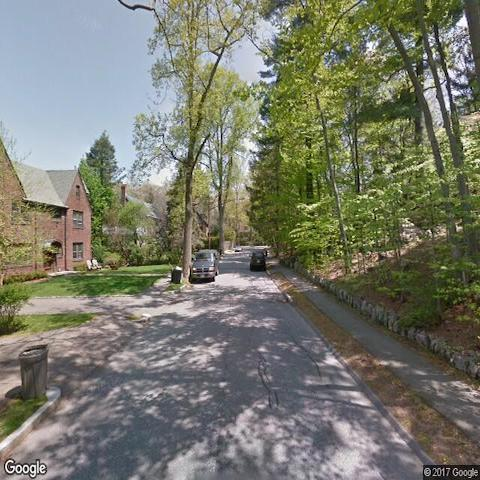
\includegraphics[width=11em]{Plot/examples/b_1} \\ 
        %		& 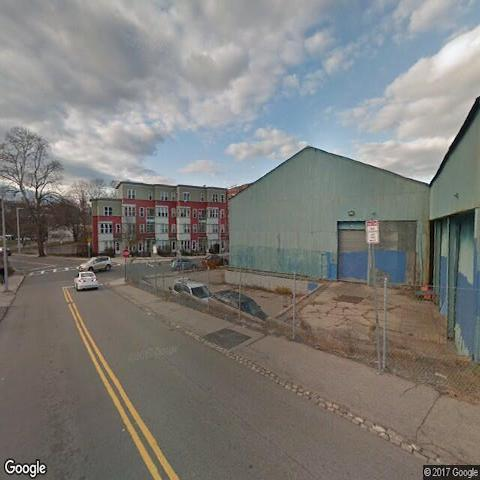
\includegraphics[width=11em]{Plot/examples/u_2} & 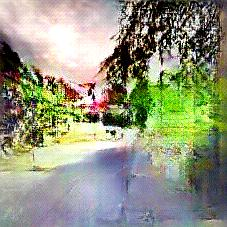
\includegraphics[width=11em]{Plot/examples/t_2} &  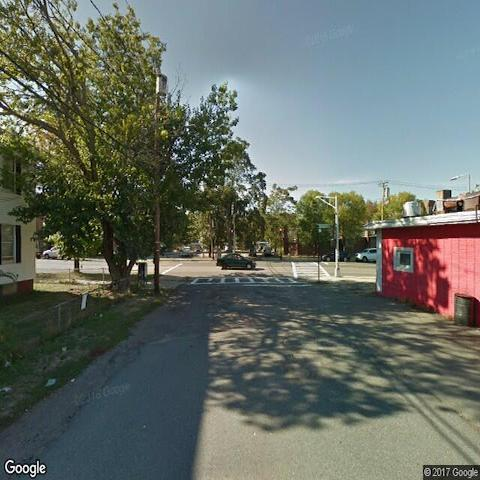
\includegraphics[width=11em]{Plot/examples/b_2} \\ 
        %		& 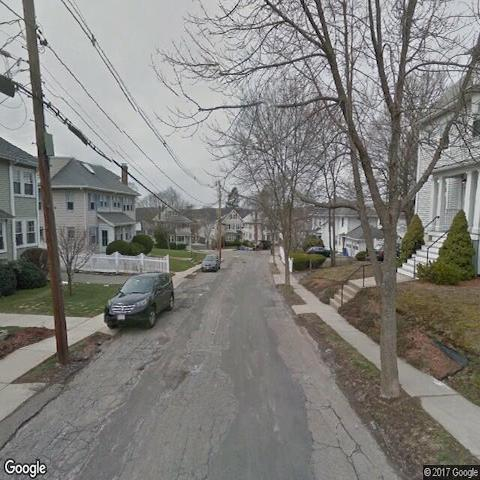
\includegraphics[width=11em]{Plot/examples/u_3} & 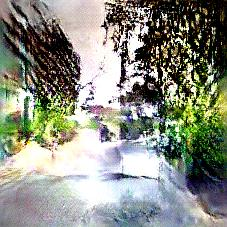
\includegraphics[width=11em]{Plot/examples/t_3} &  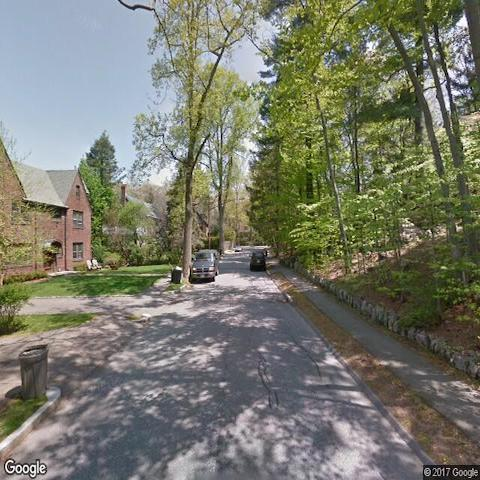
\includegraphics[width=11em]{Plot/examples/b_3} \\ 
        & 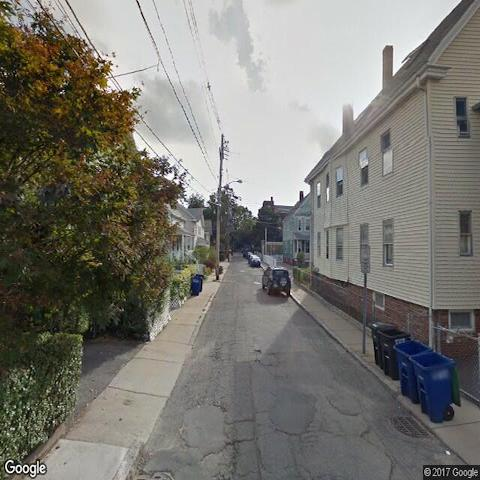
\includegraphics[width=11em]{u_4.jpeg} & 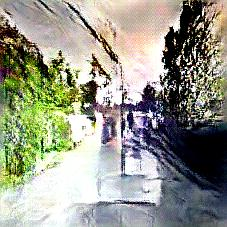
\includegraphics[width=11em]{t_4.jpeg} &  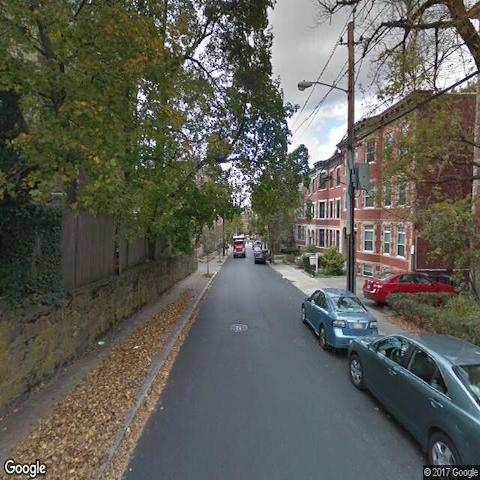
\includegraphics[width=11em]{b_4.jpeg} \\ 
        & 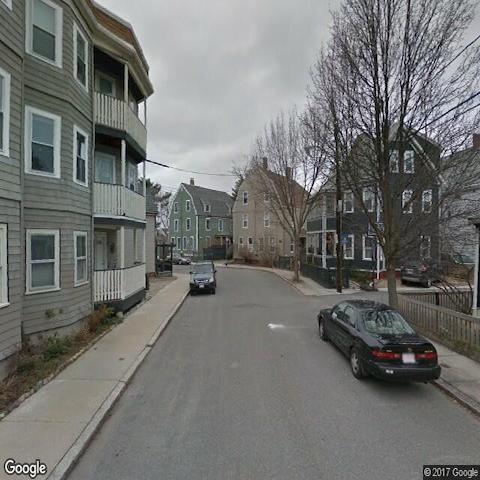
\includegraphics[width=11em]{u_5.jpeg} & 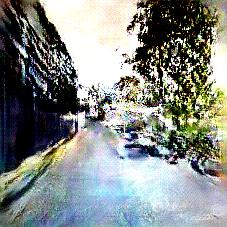
\includegraphics[width=11em]{t_5.jpeg} &  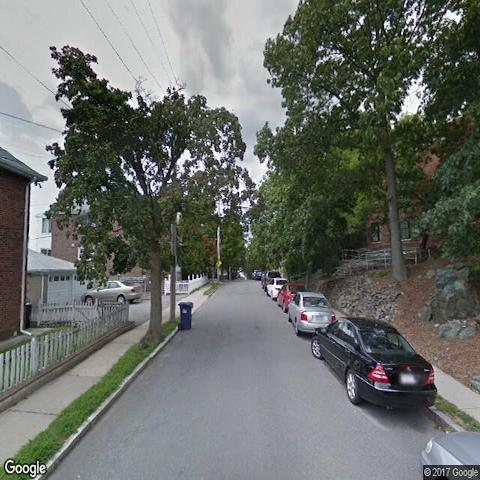
\includegraphics[width=11em]{b_5.jpeg} \\ 
        %		& 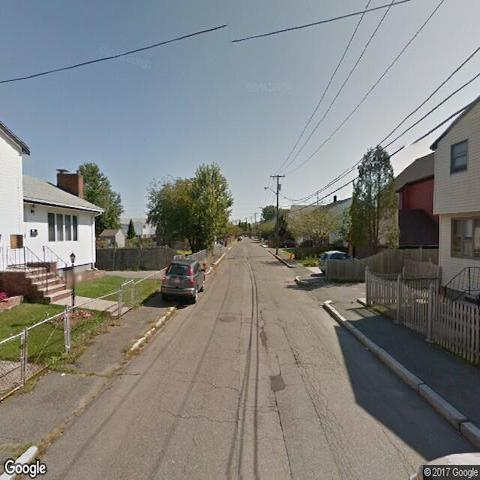
\includegraphics[width=11em]{Plot/examples/u_6} & 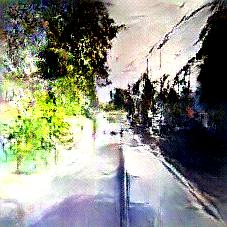
\includegraphics[width=11em]{Plot/examples/t_6} &  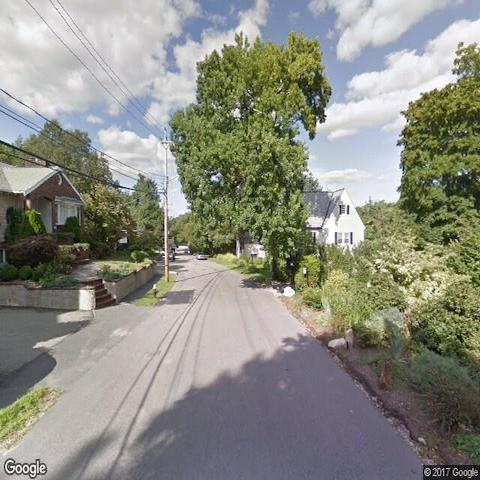
\includegraphics[width=11em]{Plot/examples/b_6} \\ 
        & 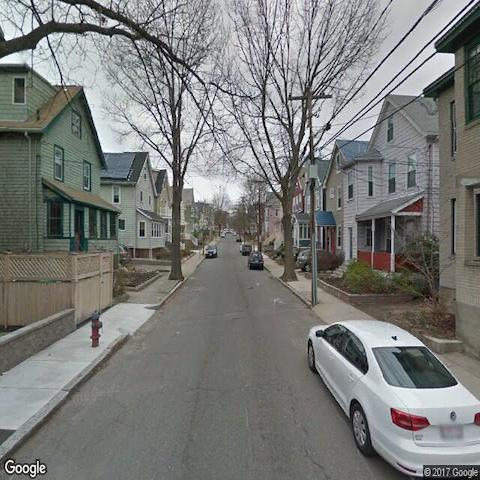
\includegraphics[width=11em]{u_7.jpeg} & 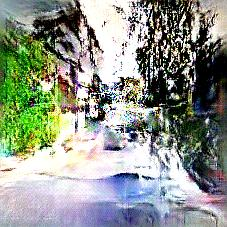
\includegraphics[width=11em]{t_7.jpeg} &  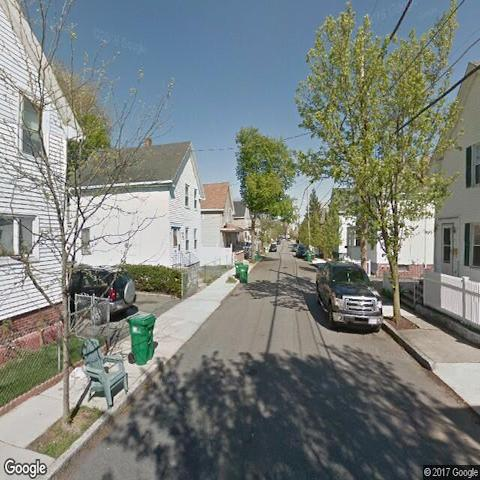
\includegraphics[width=11em]{b_7.jpeg} \\ 
        & 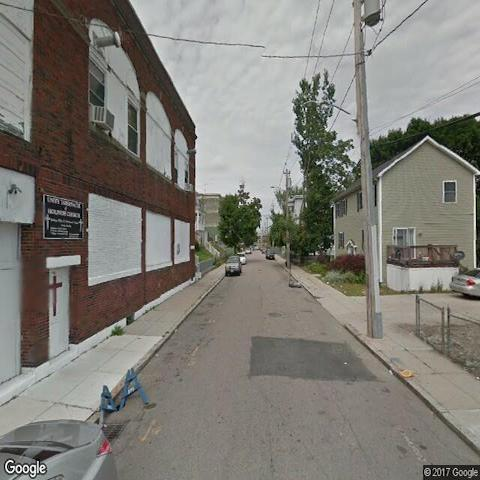
\includegraphics[width=11em]{u_8.jpeg} & 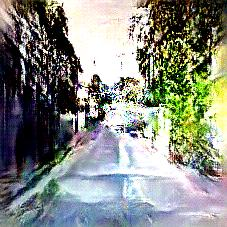
\includegraphics[width=11em]{t_8.jpeg} &  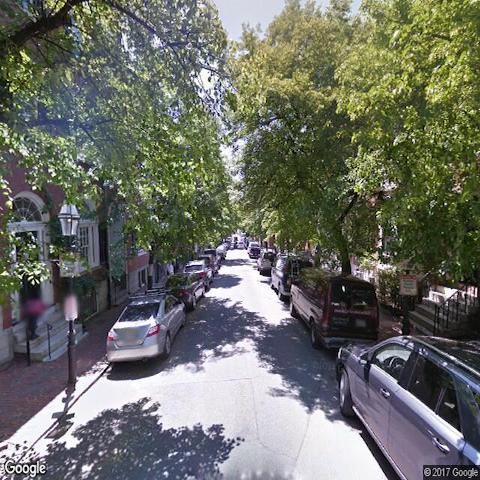
\includegraphics[width=11em]{b_8.jpeg} \\ 
        \bottomrule 
    \end{tabular}
    \caption{Examples of the ``FaceLifting'' process, which tends to add greenery, narrow roads, and  pavements.}
    \label{fig:BeautyExample}
\end{table} 




\section{Evaluation}
\label{sec:evaluation}

The goal of FaceLift is to transform existing urban scenes into versions that: \emph{i)} people perceive more beautiful; \emph{ii)} contain urban elements typical of great urban spaces; \emph{iii)} are easy to interpret; and \emph{iv)} architects and urban planners find useful. To ascertain whether FaceLift meets that composite goal, we answer the following questions next: 

\begin{description}
    \item{\textbf{Q1}} Do individuals perceive ``FaceLifted'' scenes to be beautiful?
    \item{\textbf{Q2}}  Does our framework produce scenes that possess urban elements typical of great spaces?  
    \item{\textbf{Q3}}  Which urban elements are mostly associated with beautiful scenes?    
    \item{\textbf{Q4}}  Do architects and urban planners find FaceLift's insights useful?    
\end{description}


\subsection{Q1 People's perceptions of beautified scenes}
To ascertain whether ``FaceLifted'' scenes are perceived by individuals as they are supposed to, we run a crowd-sourcing experiment on Amazon Mechanical Turk.  We randomly select 200 scenes, 100 beautiful and 100 ugly  (taken at the bottom 10 and top 10 percentiles of the Trueskill's score distribution of Figure~\ref{fig:Trueskill}). Our framework then transforms each ugly scene into its beautified version, and each beautiful scene into its corresponding `uglified'. These scenes are arranged into pairs, each of which contains the original scene and its beautified or uglified version. On  Mechanical Turk, we only select verified masters as our crowd-sourcing workers (those with an approval rate above 90\% during the past 30 days), pay them \$0.1 per  task,  and ask each of them to choose the most beautiful scene for each given pair.  We make sure to have at least 3 votes for each scene pair. Overall, our workers end up selecting the scenes that are actually beautiful 77.5\% of the times, suggesting that ``FaceLifted'' scenes are indeed perceived to be more beautiful by people. 

\subsection{Q2 Are beautified scenes great urban spaces?}
To answer that question, we need to understand what makes a space great. After reviewing the literature in urban planning, we identify four factors associated with  great places~\cite{ewing2013measuring,alexander1977pattern} (Table~\ref{tab:Design_metrics}): they mainly tend to be walkable, offer greenery, feel cozy, and be visually rich. 

\begin{table*}[h]
    \centering
    
    \resizebox{\linewidth}{!}{%
        \begin{tabular}{|c|p{10cm}|}
            \hline
            \textbf{Metric} & \textbf{Description}\\
            \hline
            Walkability  & Walkable streets support people's natural tendency to explore spaces~\cite{ewing2013measuring,quercia15thedigital,speck12}.\\
            \hline
            Green Spaces & The presence of greenery has repeatedly been found to impact people's well-being \cite{alexander1977pattern}. Under certain conditions, it could also promote social interactions~\cite{quercia2014aesthetic}. Not all types of greenery have to be considered the same though: dense forests or unkempt greens might well have a negative impact~\cite{jacobs1961death}. \\
            \hline		
            Landmarks & Feeling lost is not a pleasant experience, and the presence of landmarks  have been shown to contribute to the legibility and navigability of spaces~\cite{lynch1960image,quercia2014aesthetic,ewing2013measuring,quercia13maps}.\\
            \hline
            Privacy-Openness & The sense of privacy conveyed by a place's structure (as opposed to a sense of openness) impacts its perception~\cite{ewing2013measuring}.\\ 
            \hline
            Visual Complexity & Visual complexity is a measure of how diverse an urban scene is in terms of design materials, textures, and objects~\cite{ewing2013measuring}. The relationship between complexity and preferences generally follows an  `inverted-U' shape: we prefer places of medium complexity rather than places of low or high complexity~\cite{ulrich1983aesthetic}. \\
            \hline
    \end{tabular}}
    \caption{Urban Design Metrics}
    \label{tab:Design_metrics}
    %        \vspace{-5mm}
\end{table*}


To automatically extract visual cues related to these four factors, we select 500 ugly scenes and 500 beautiful ones at random, transform them into their opposite aesthetic qualities (i.e., ugly ones are beautified, and beautiful ones are `uglified'), and compare which urban elements related to the four factors distinguish uglified scenes from beautified ones. 

We extract labels from each of our 1,000 scenes using two image classifiers. First, using PlacesNet~\cite{zhou2014learning}, we label each of our scenes according to a classification containing 205 labels (reflecting, for example, landmarks, natural elements), and retain the five labels with highest confidence scores for the scene. We then manually classify these 205 labels into the 4 built environment types namely \textit{Walkable, Architectural, Natural and Landmark}. These types are inspired by the guidelines for measuring urban design~\cite{ewing2013measuring}. The specifics of their category definitions and the actual labels can be seen in Appendix 2(Chapter ~\ref{chap:app2}).  Second, using Segnet~\cite{badrinarayanan2015segnet}, we  label each of our scenes according to a classification containing 12 labels. Segnet is trained on dash-cam images, and classifies each scene pixel with one of these twelve labels: road, sky, trees,  buildings, poles, signage, pedestrians, vehicles, bicycles, pavement, fences, and road markings. 

\begin{figure}[h]
    \centering
    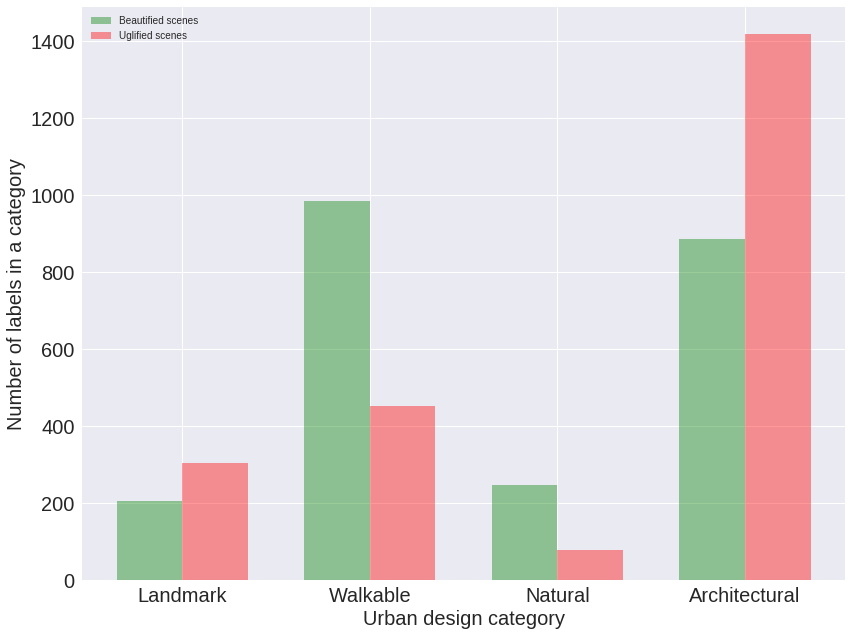
\includegraphics[width=\columnwidth]{taxonomyCount.png}
    \caption{Number of labels in specific urban design categories (on the $x$-axis) found in beautified scenes as opposed to those found in uglified scenes.}
    \label{fig:taxonomyCount}
\end{figure}


\begin{figure}[h]
    \centering
    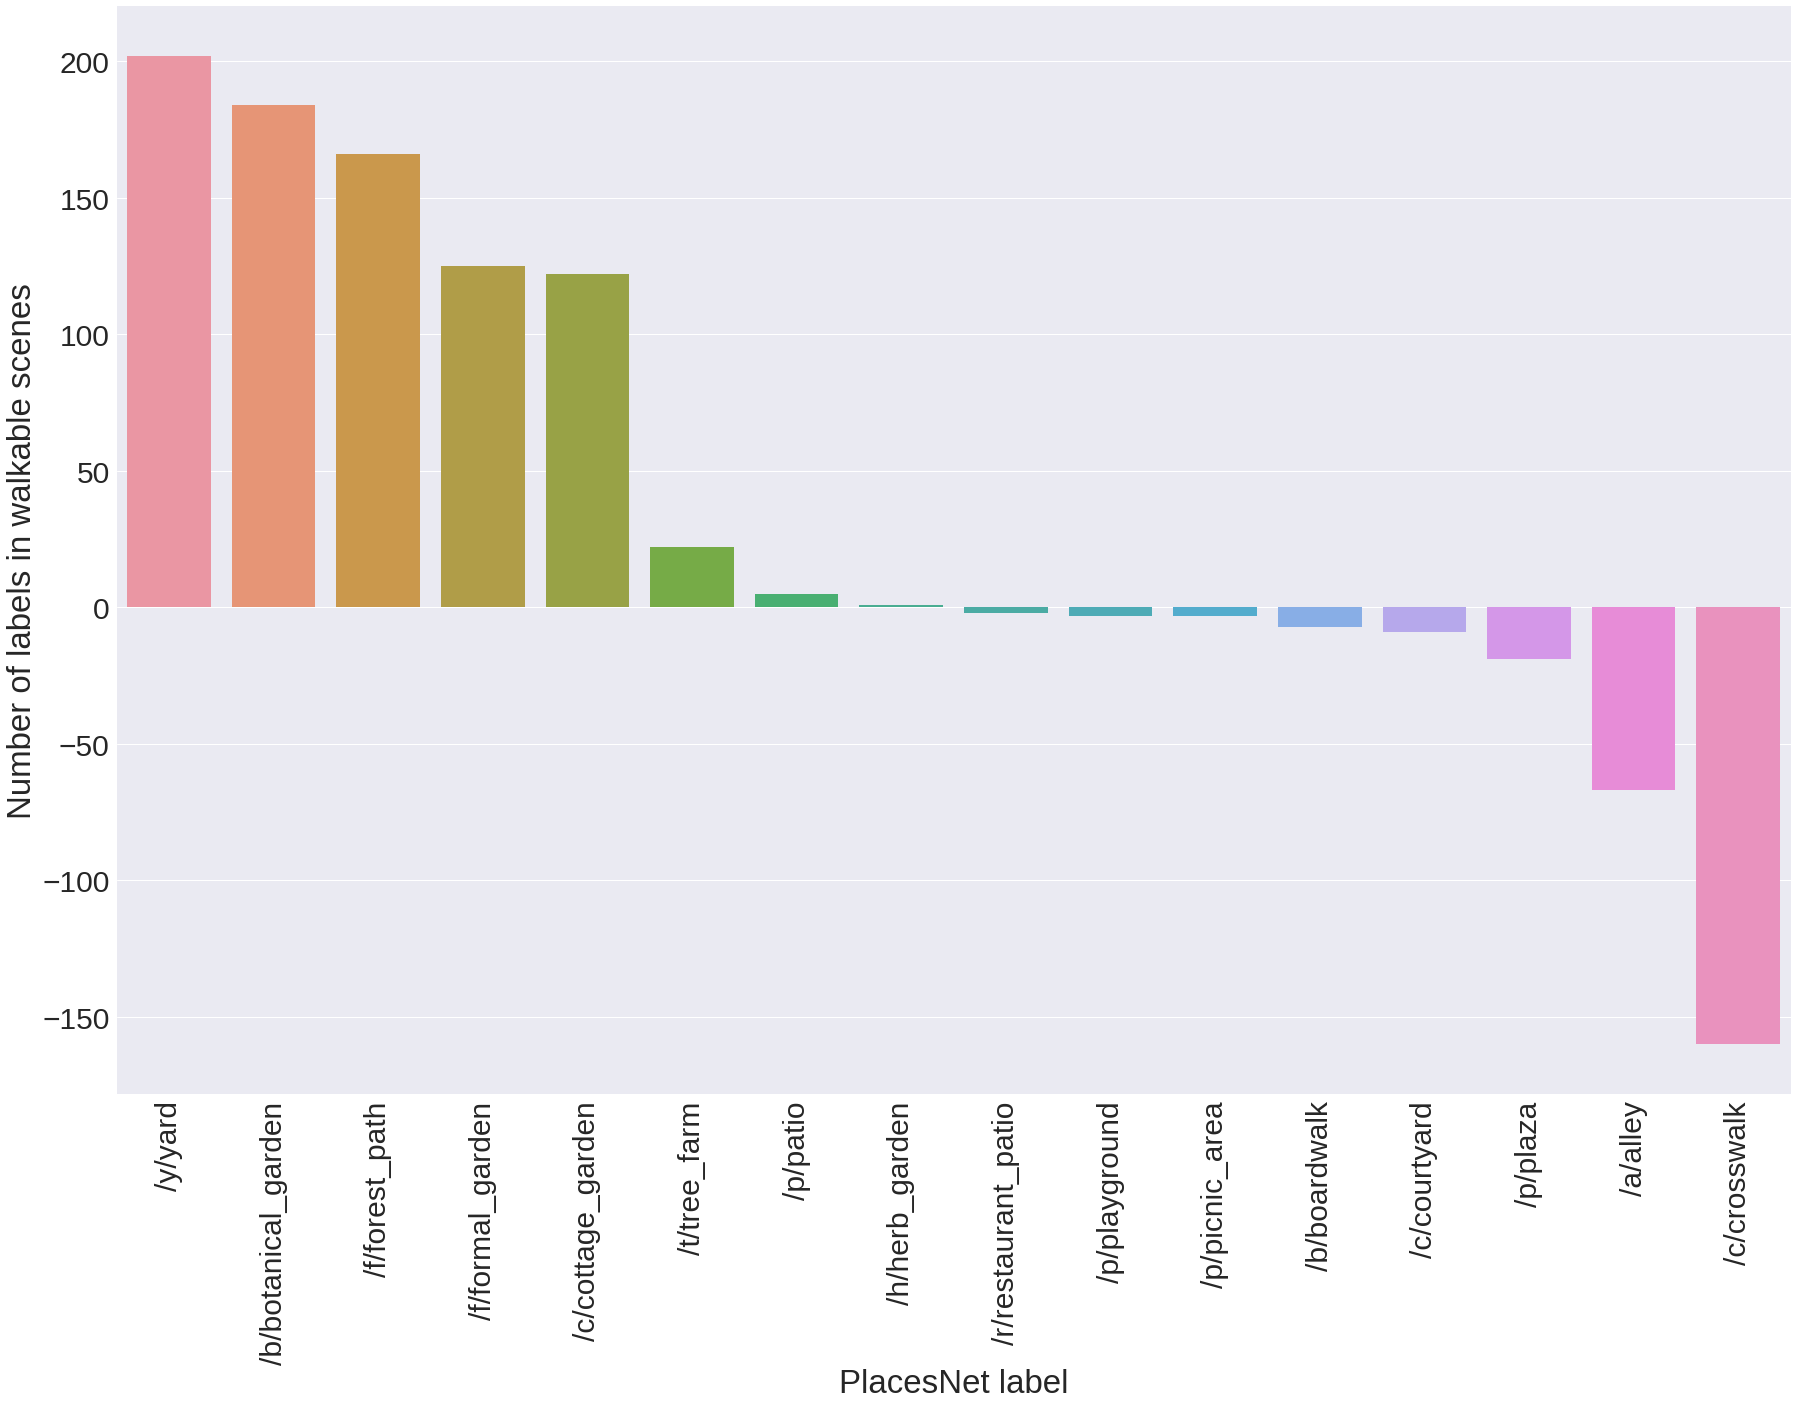
\includegraphics[width=\columnwidth]{walkable_taxonomy.png}
    \caption{Count of specific walkability-related labels  (on the $x$-axis) found in beautified scenes minus the count of the same labels found in uglified scenes.}
    \label{fig:WalkableTnomy}
\end{figure}


Having these two ways of labelling scenes, we can now test whether the expectations set by the literature describing metrics of great urban spaces (Table~\ref{tab:Design_metrics}) are  met in the Face-lifted scenes. 


%**************************************************
\mbox{ } \\
\noindent
\emph{H1 Beautified scenes tend to be walkable.}
We manually select only the PlacesNet labels that are related to walkability. These labels include, for example, \textit{abbey, plaza, courtyard, garden, picnic area, \textrm{and} park}. To test hypothesis \emph{H1}, we count the number of walkability-related labels found in beautified scenes as opposed to those found in uglified scenes (Figure~\ref{fig:taxonomyCount}): the former contain twice as many walkability labels than the latter. We then determine which types of scenes are associated with beauty (Figure~\ref{fig:WalkableTnomy}). Unsurprisingly, beautified scenes tend to show gardens, yards, and small paths. By contrast, uglified ones tend to show built environment features such as shop fronts and broad roads. 


\mbox{ } \\
%**************************************************
\noindent
\emph{H2 Beautified scenes tend to offer green spaces.}
We manually select only the PlacesNet labels that are related to greenery. These labels include, for example, \textit{fields, pasture, forest, ocean, and beach}. Then, in our 1,000 scenes, to test hypothesis \emph{H2}, we count the number of nature-related labels found in beautified scenes as opposed to those found in uglified scenes (Figure~\ref{fig:taxonomyCount}): the former contain more than twice as many nature-related labels than the latter.  To test this hypothesis further, we compute the fraction of `tree' pixels (using SegNet's label `tree') in beautified and uglified scenes, and  find that beautification adds  32\% of tree pixels, while uglification removes 17\% of them. 


\begin{figure*}[!t]
    \centering
    \hspace*{-5mm}
    \subfloat[]{
        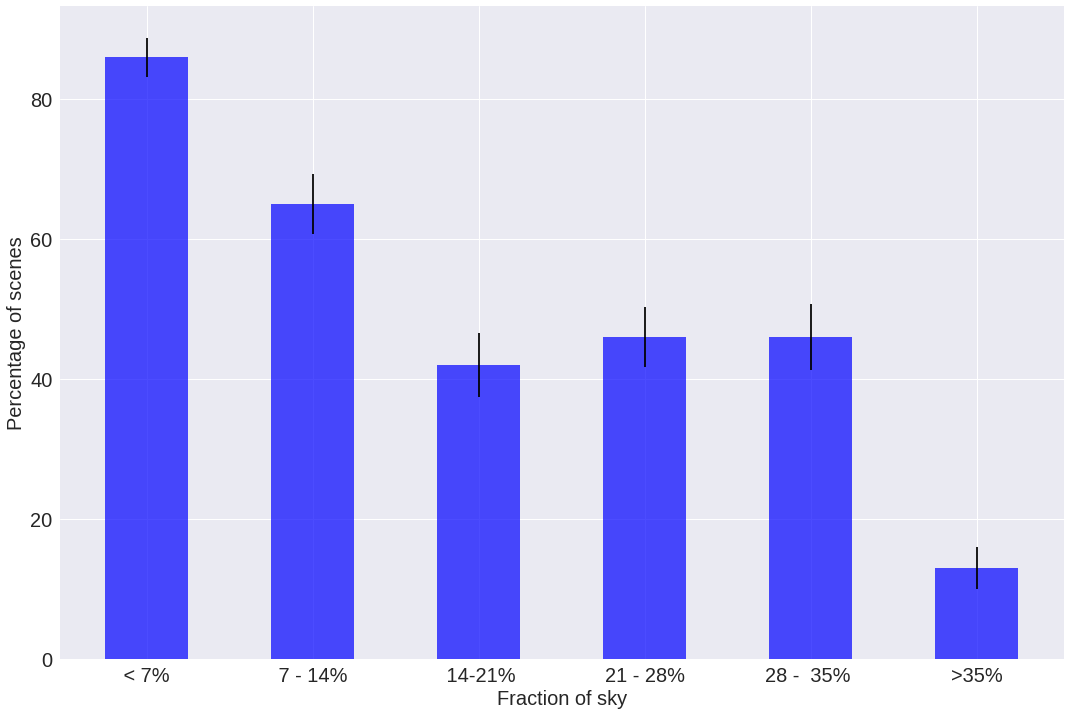
\includegraphics[width=0.45\textwidth, height = 5cm ]{BinnedPlot.png}
        \label{fig:skyBinned}
    }
    \subfloat[]{
        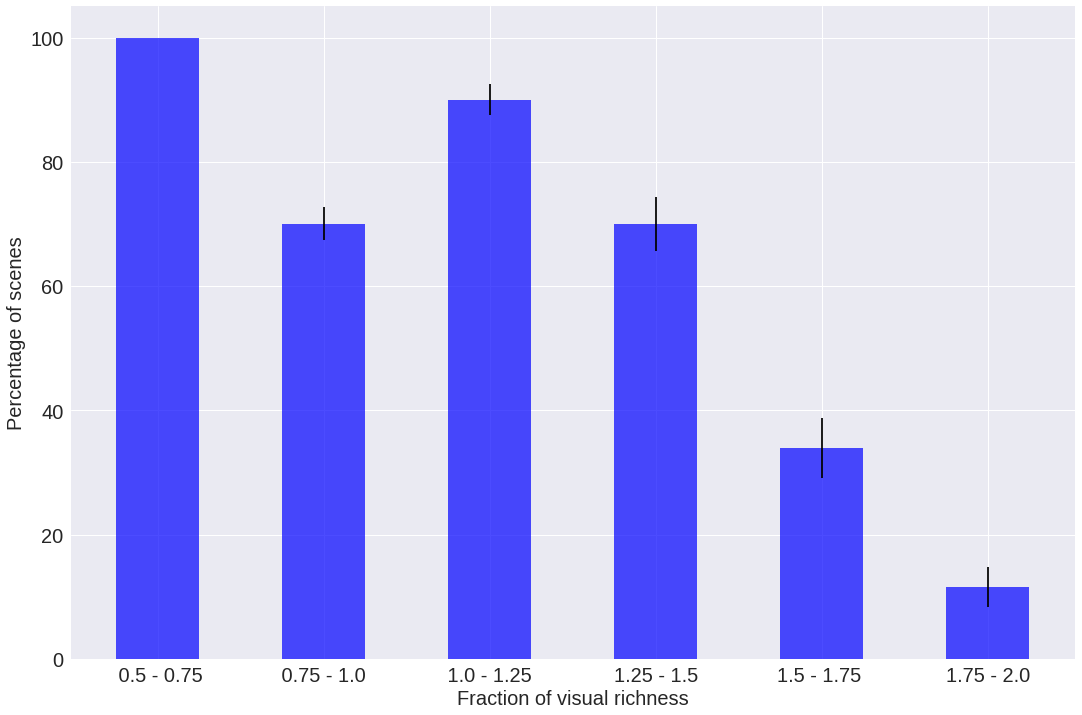
\includegraphics[width=0.45\linewidth, height = 5cm ]{binnedPlot_complexity.png}
        \label{fig:complexity}
    }
    \vspace{-0.4cm}
    \label{fig:bin_figures}
    \caption{The percentage of beautified scenes ($y$-axis): (a) having an increasing presence of sky (on the $x$-axis); and (b) having an increasing level of visual richness  (on the $x$-axis). The error bars represent standard errors obtained by random re-sampling of the data for 500 iterations. }
    \vspace{-0.4cm}
\end{figure*}



\mbox{ } \\
%**************************************************
\noindent
\emph{H3 Beautified scenes tend to feel private and `cozy'.}
To  test hypothesis \emph{H3}, we count the fraction of pixels that Segnet labeled  as `sky' and show the results in a bin plot in Figure~\ref{fig:skyBinned}:  the $x$-axis has six bins (each of which represents a given range of sky fraction), and the $y$-axis shows the percentage of beautified \emph{vs.} uglified scenes that fall into each bin.  Beautified scenes tend to be cozier (lower sky presence) than the corresponding original scenes.


\mbox{ } \\
%**************************************************
\noindent
\emph{H4 Beautified scenes tend to be visually rich.}
To quantify to which extent scenes are visually rich, we measure their visual complexity~\cite{ewing2013measuring} as  the amount of disorder in terms of distribution of (Segnet) urban elements in the scene: 
\begin{equation}
H(X) = -\sum p(i)\log p(i)
\label{eq:entropy} 
\end{equation}
where $i$ is the $i^{th}$ Segnet's label. The total number of labels is twelve. The higher $H(X)$, the  higher the scene's entropy, that is, the higher the scene's complexity. It has been suggested that the relationship between complexity and  pleasantness follows an `inverted U' shape~\cite{ulrich1983aesthetic}: we prefer places of medium complexity rather than places of low or high complexity. To test that, we show the percentage of beautified scenes that fall into each complexity bin  (Figure~\ref{fig:complexity}):  we do not find a strong evidence of the `inverted U' shape hypothesis, in that, beautified scenes are of low to medium complexity, while uglified ones are of high complexity.



%**************************************************
\subsection{Q3 Urban elements of beautified scenes}

\begin{table}[t!]
    \centering
    \resizebox{\linewidth}{!}{%
        \begin{tabular}{|c|c|c|c|c|}
            \hline
            \textbf{Pair of urban elements} & \textbf{$\beta_1$}  & \textbf{$\beta_2$} & \textbf{$\beta_3$}  & Error Rate (Percentage)\\
            \hline
            \hline
            Buildings - Trees & -0.032 & 0.084  & 0.005  & 12.7 \\
            \hline
            Sky - Buildings & -0.08 & -0.11 & 0.064 & 14.4 \\
            \hline
            Roads - Vehicles  & -0.015  & -0.05 & 0.023  & 40.6 \\
            \hline
            Sky - Trees & 0.03 & 0.11 & -0.012 & 12.8  \\
            \hline
            Roads - Trees & 0.04  & 0.10 &  -0.031  & 13.5  \\
            \hline
            Roads - Buildings & -0.05  & -0.097  &  0.04  & 20.2  \\
            \hline
        \end{tabular}
    }
    \caption{Coefficients of logistic regressions run on one pair of predictors at the time.}
    \label{tab:regressioncoef}
    \vspace{-10mm}
\end{table}


To determine which urban elements are the best predictors of urban beauty and the extent to which they are so, we run a logistic regression, and, to ease interpretation, we do so on one pair of predictors at the time: 
\begin{equation}
Pr(\textrm{beautiful}) = logit^{-1}(\alpha + \beta_1 * V_1 + \beta_2 * V_2  + \beta_3 * V_{1}.V_{2} )
\label{eq:regression} 
\end{equation}
where $V1$ is the fraction of the scene's pixels marked with one Segnet's label, say, ``buildings'' (over the total number of pixels),  and $V2$ is the fraction of the scene's pixels marked with another label, say, ``trees''. The result consists of three beta coefficients: $\beta_1$ reflects $V1$'s contribution in predicting beauty,  $\beta_2$ reflects $V2$'s contribution, and $\beta_3$ is the interaction effect, that is, it reflects the contribution of the dependency between $V1$ and $V2$ in predicting beauty. We run logistic regressions on the five factors that have been found to be most predictive of urban beauty~\cite{quercia2014aesthetic, ewing2013measuring, alexander1977pattern}, and show the results in Table~\ref{tab:regressioncoef}.


Since we are using logistic regressions, the quantitative interpretation of the beta coefficients is eased by the ``divide by 4 rule''~\cite{vaughn2008data}: we can take the $\beta$ coefficients and ``divide them by 4 to get an upper bound of the predictive difference corresponding to a unit difference'' in beauty~\cite{vaughn2008data}. For example, take the results in the first row of Table~\ref{tab:regressioncoef}. In the model $Pr(beautiful) = logit^{-1}(\alpha - 0.032 \cdot buildings + 0.084 \cdot trees + 0.005 \cdot  buildings \cdot trees)$, we can divide - 0.032/4 to get -0.008: a difference of 1 in the fraction of pixels being buildings corresponds to no more than a 0.8\% \emph{negative} difference in the probability of the scene being beautiful. In a similar way, a difference of 1 in the fraction of pixels being trees corresponds to no more than a 0.021\% \emph{positive} difference in the probability of the scene being beautiful. By considering the remaining results in Table~\ref{tab:regressioncoef}, we find that, across all pairwise comparisons, trees is the most positive element associated with beauty, while roads and buildings are the most negative ones. These results match previous literature in urban design of what makes spaces great, adding further external validity to our framework's beautification. 




%**************************************************
\subsection{Q4 Do architects and urban planners find it useful?}

\begin{figure}[ht]
    \centering
    \includegraphics[width=\linewidth]{facelift-pipeline-2x.png}
    \caption{An end to end illustration of the FaceLift framework.}
    \label{fig:framework}
\end{figure}


\begin{table}[t!]
    \centering
    \resizebox{\linewidth}{!}{%
        \begin{tabular}{|c|c|c|c|c|c|}
            \hline
            \textbf{Use case} & \textbf{Definitely Not}  & \textbf{Probably Not} & \textbf{Probably}  & \textbf{Very Probably} & \textbf{Definitely}\\
            \hline
            \hline
            Decision Making & 4.8\% & 9.5\%  & 38\%  &  28.6\% & 19\%\\
            \hline
            Participatory Urban Planning & 0\% & 4.8\%  & 52.4\%  &  23.8\% & 19\%\\
            \hline
            Promote Green Cities & 4.8\% & 0\%  & 47.6\%  &  19\% & 28.6\%\\
            \hline
        \end{tabular}
    }
    \caption{Urban experts polled about the extent to which an interactive map of ``FaceLifted'' scenes promotes: (a) decision making; (b) citizen participation in urban planning; and (c) promotion of green cities}
    \label{tab:useCases}
    \vspace{-10mm}
\end{table}


%\begin{figure*}[!t]
%	\centering
%	\hspace*{-5mm}
%	\subfloat[]{
%		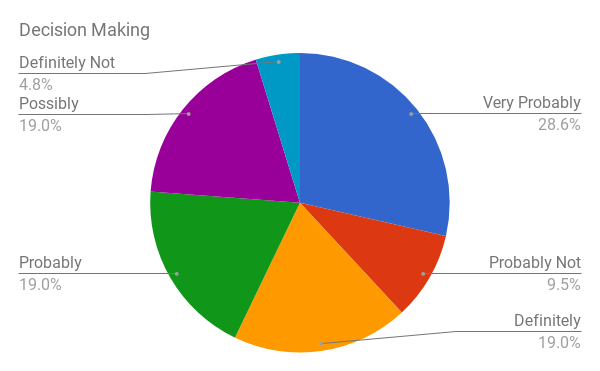
\includegraphics[width=0.3\textwidth ]{Plot/DecisionMaking.png}
%		\label{fig:decision}
%	}
%	\subfloat[]{
%		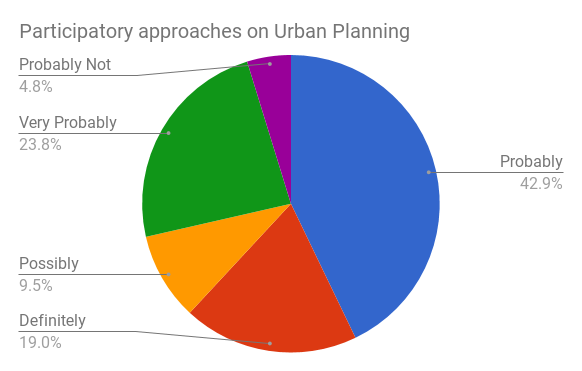
\includegraphics[width=0.3\linewidth ]{Plot/ParticipationUrbanPlanning.png}
%		\label{fig:participation}
%	}
%	\subfloat[]{
%		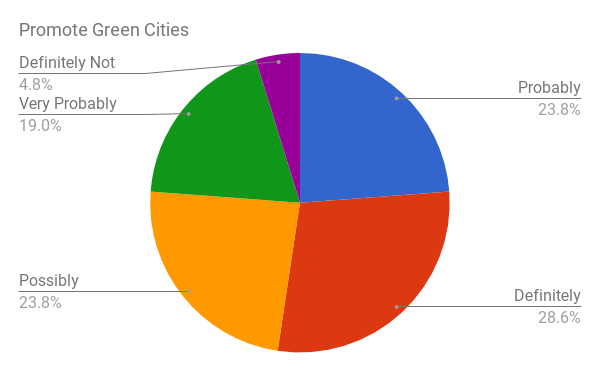
\includegraphics[width=0.3\linewidth ]{Plot/PromoteGreenCities.png}
%		\label{fig:promotion}
%	}
%%	\vspace{-0.4cm}
%	\caption{Urban experts polled about the extent to which an interactive map of ``FaceLifted'' scenes promotes: (a) decision making; (b) citizen participation in urban planning; and (c) promotion of green cities.\ns{Pie charts are not advisible. The labels are too small. You can perhaps replace this with a table.}}
%	\label{fig:pies}
%	\vspace{-0.4cm}
%\end{figure*}


\begin{figure}[t!]
    \centering
    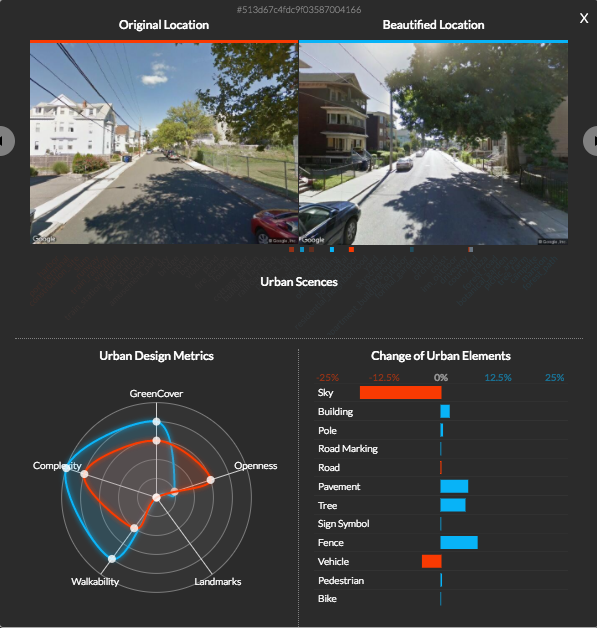
\includegraphics[width=\columnwidth]{UI.png}
    \caption{Interactive visualization of FaceLifted scenes in Boston}
    \label{facelift-UI}
\end{figure}


To ascertain whether practitioners find FaceLift potentially useful, we build an interactive map of the city of Boston in which, for  selected points, we show pairs of urban scenes before/after beautification (Figure~\ref{facelift-UI})\footnote{It is worth noting that the visualization is not claimed to be my original contribution. The design of the interactive map was done by the first author of article~\ref{IEEE}}. We then send that map along with a survey to 20 experts in architecture, urban planning, and data visualization around the world. Questions were asked with a non-neutral response Likert scale (Table~\ref{tab:useCases}). That is because previous work~\cite{Agree2012,moors2008exploring} has shown that such a scale: \emph{(i)} pushes respondents to ``take a stance'', given the absence of a neutral response; and \emph{(ii)} works best if respondents are experts in the subject matter of the survey as responses of the ``I don't know'' type tend to be rare (as it is has been the case for our survey). The experts had to complete tasks in which they rated FaceLift based on how well it supports decision making, participatory urbanism, and the promotion of green spaces. According to our experts (Table~\ref{tab:useCases}), the tool can very probably supports decision making, probably support participatory urbanism, and definitely promote green spaces.  These results are  also qualitatively supported by our experts' comments, which include: ``\textit{The maps reveal patterns that might not otherwise be apparent}'',  ``\textit{The tool helps focusing on parameters to identify beauty in the city while exploring it}'',  and ``\textit{The metrics are nice. It made me think more about beautiful places needing a combination of criteria, rather than a high score on one or two dimensions. It made me realize that these criteria are probably spatially correlated}''.






\section{Conclusion}
\label{sec:discussion}

FaceLift is a  framework that automatically beautifies urban scenes by combining recent approaches of Generative Adversarial Networks and Deep Convolutional Networks. To make it usable by practitioners, the framework is also able to explain which urban elements have been added/removed during the beautification process. 

There are still important limitations though. One is data bias. The framework is as good as its training data, and more work has to go into collecting reliable ground truth data on human perceptions. This data should ideally be stratified according to the people's characteristics that  impact their perceptions. The other main limitation is that generative models are hard to control, and more work has to go into offering principled ways of fine-tuning the generative process.

Despite these limitations, FaceLift has the potential to support urban interventions  in scalable  and replicable ways: it can be applied to an entire city (scalable), across a variety of cities (replicable). To turn existing spaces into something more beautiful, that will still be the duty of architecture. Yet, with technologies similar to FaceLift more readily available, the complex job of recreating restorative spaces in an increasingly urbanized world will be greatly simplified.  


After all, ``we delight in complexity to which genius have lent an appearance of simplicity.''~\cite{de2008architecture} In the context of future work, that genius is represented by future technologies that will help us deal with the complexity of our cities.



\subsection{Limitations and biases}
Like any supervised deep learning based framework, this work is only able to learn what is present in the data. Hence the method of acquiring annotations  for urban images can introduce huge biases in the model. The current model is trained on images acquired from the study on streetscore \cite{naik2014streetscore}. However their annotation is open to general public and there is not way we can remove biases that come with culture and location, in a highly subjective effect like beauty. Moreover because the pair wise choice is simply done by clicking one of the two images, the data might have noise introduced by non-serious participants. Such biases are bound to be picked up by the deep learning model. One can argue that the preference of our model for greenery , is a form of bias in the data. Another bias introduced because of data is the model's lack of preference to pedestrians. This bias was established well in advance because Google tries to remove most of the people from their street view images for privacy reasons. Hence people, which make up a major aspect of urban vitality, are completely missing from most dataset images and hence from the facelift transformations. 
Another Limitation of our work is in the metric formation. The computational metrics developed to capture the real urban design metrics are designed using heuristics. There needs to be more crowd and expert validation to establish the validity of their formulation. 
%
\subsection{Implications}
In the works through my Ph.D., the idea of quantifying the subjective has always been the central theme. The subjective is where most of our human existence takes place. As Emanuel Kant instructs, ``Look closely, the beautiful may be small''. And indeed, the insights that drive the quantification of beauty in this part of my work, seem to be almost intuitive. Greenery, walking spaces and open spaces seem drive our perception of the aesthetic, which may be grounded in our natural roots and evolutionary need to be safe and close to nature. Despite of the root causes seeming intuitive, the implications of these simple properties of urban spaces on mental and physical health seem to be far more crucial in today's world. 
At such a juncture, it is worth while to develop these frameworks to capture human subjective experiences. Thankfully because of the convergence in our online and offline lives, we are generating far more data about our offline experiences, online. Data acquired from how we interact with different on-line services, may very well improve our off-line lives.